\chapter{Results}
\label{chap:results}


\section{Rotation estimation}

% \begin{figure}[H] 
%   \centering
%   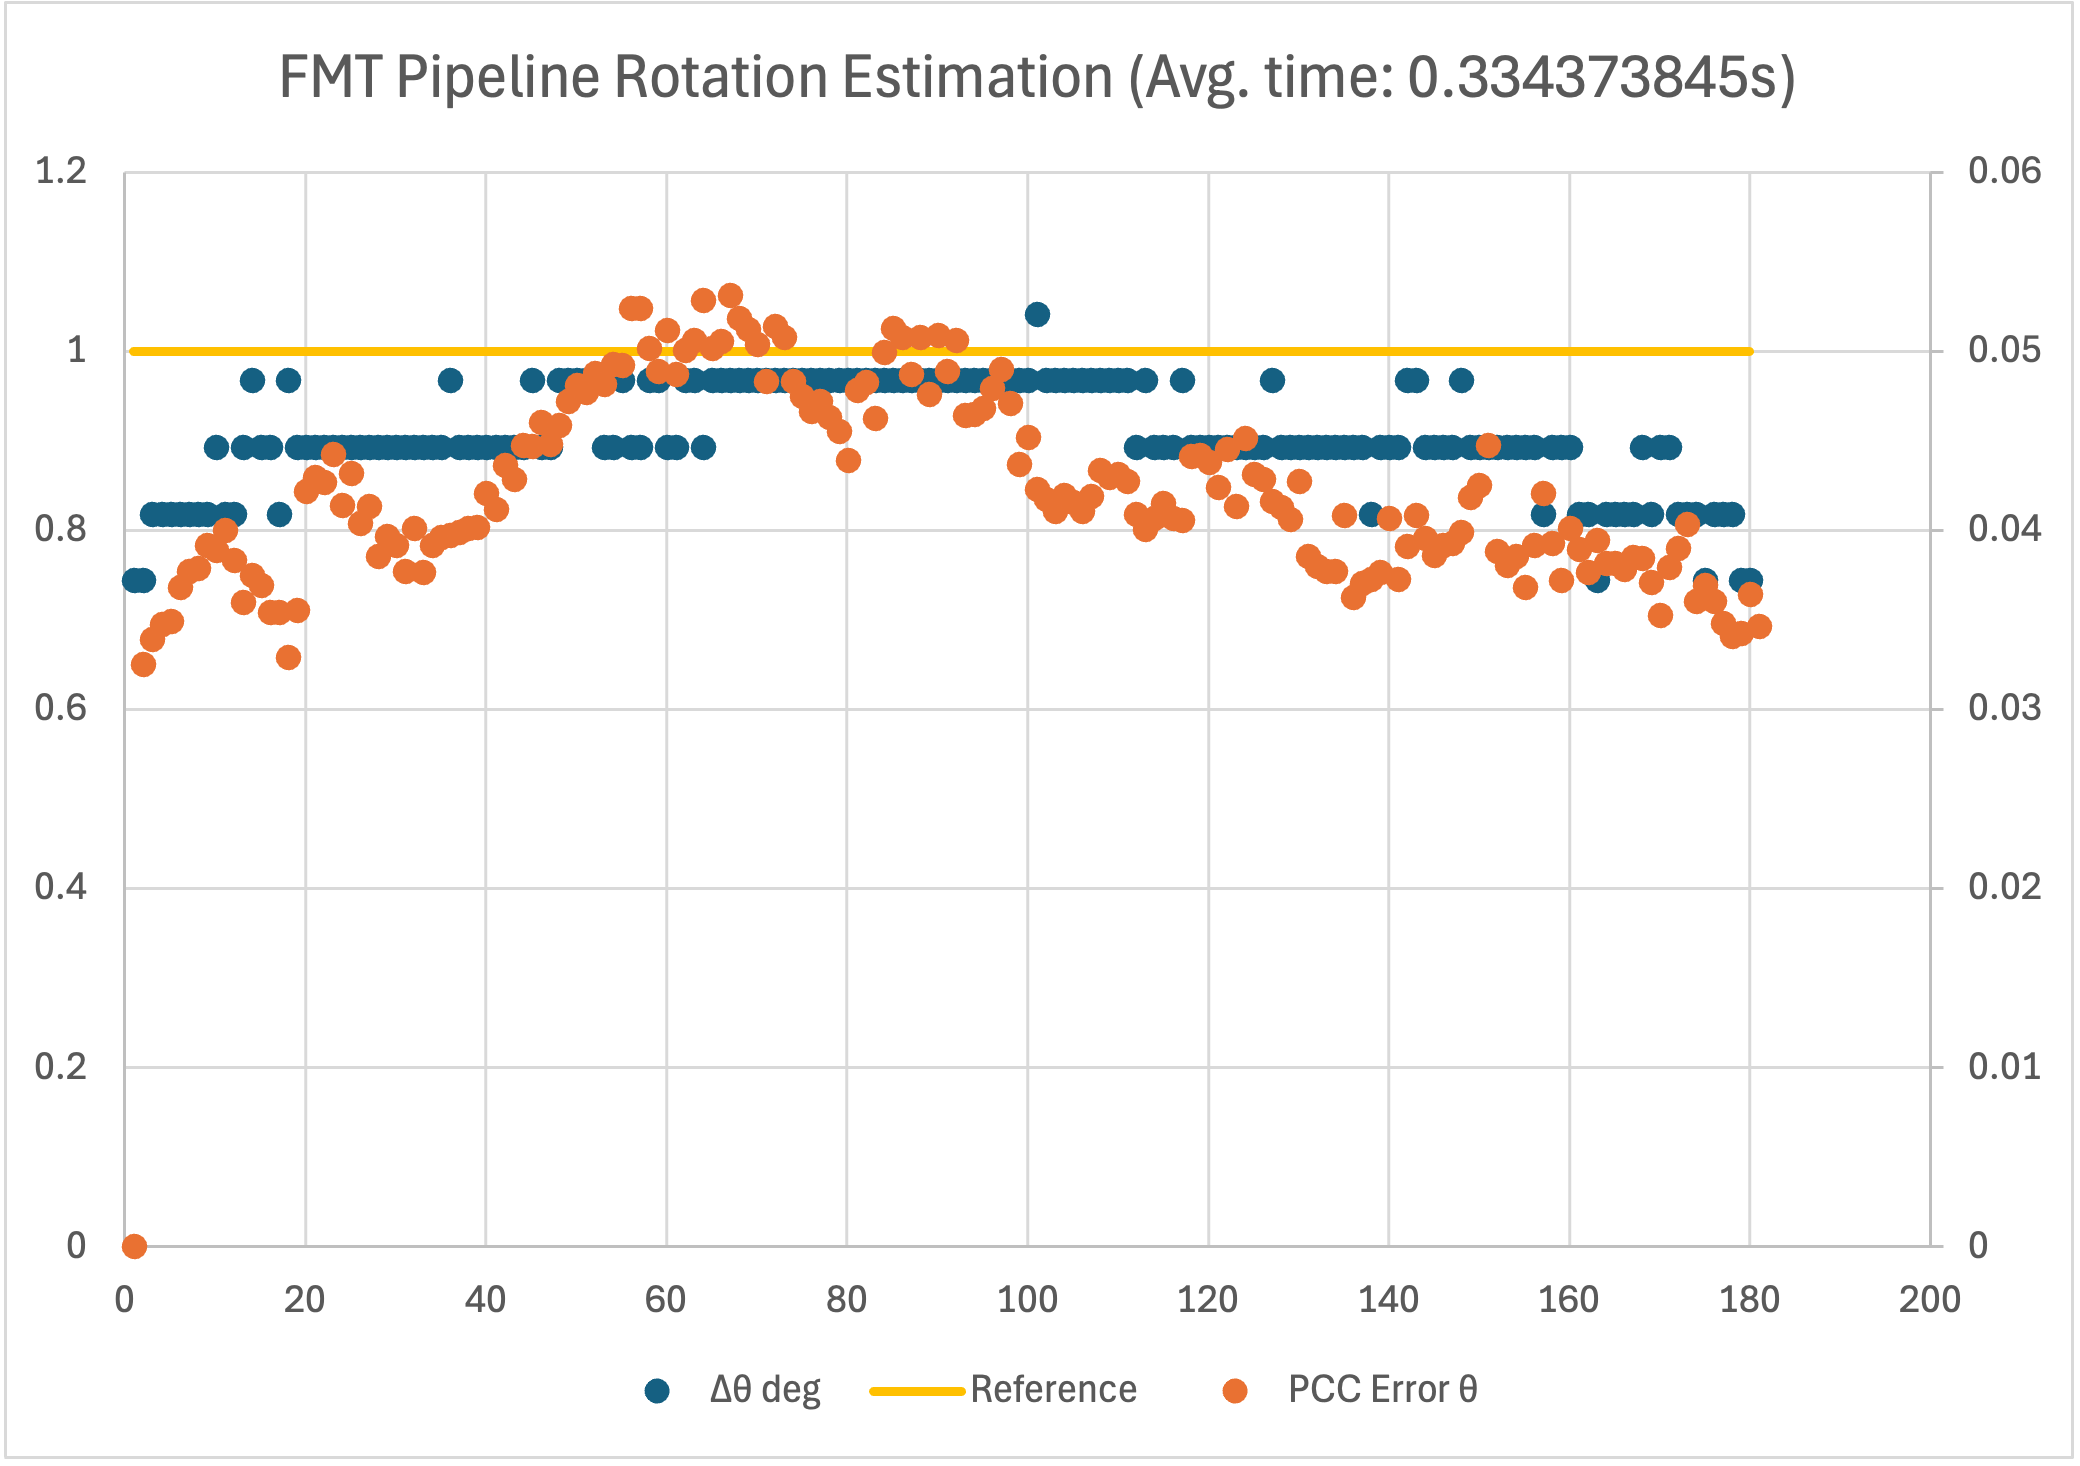
\includegraphics[width=.7\textwidth]{figures/results/rotation-skip-0/FMT-Rotation.png}
%   \caption[Fourier-Mellin Pipeline Rotation Estimation]{Rotation estimation using the Fourier-Mellin Pipeline}
%   \label{fig:fmrotation}
% \end{figure}


% \begin{figure}[H] 
%   \centering
%   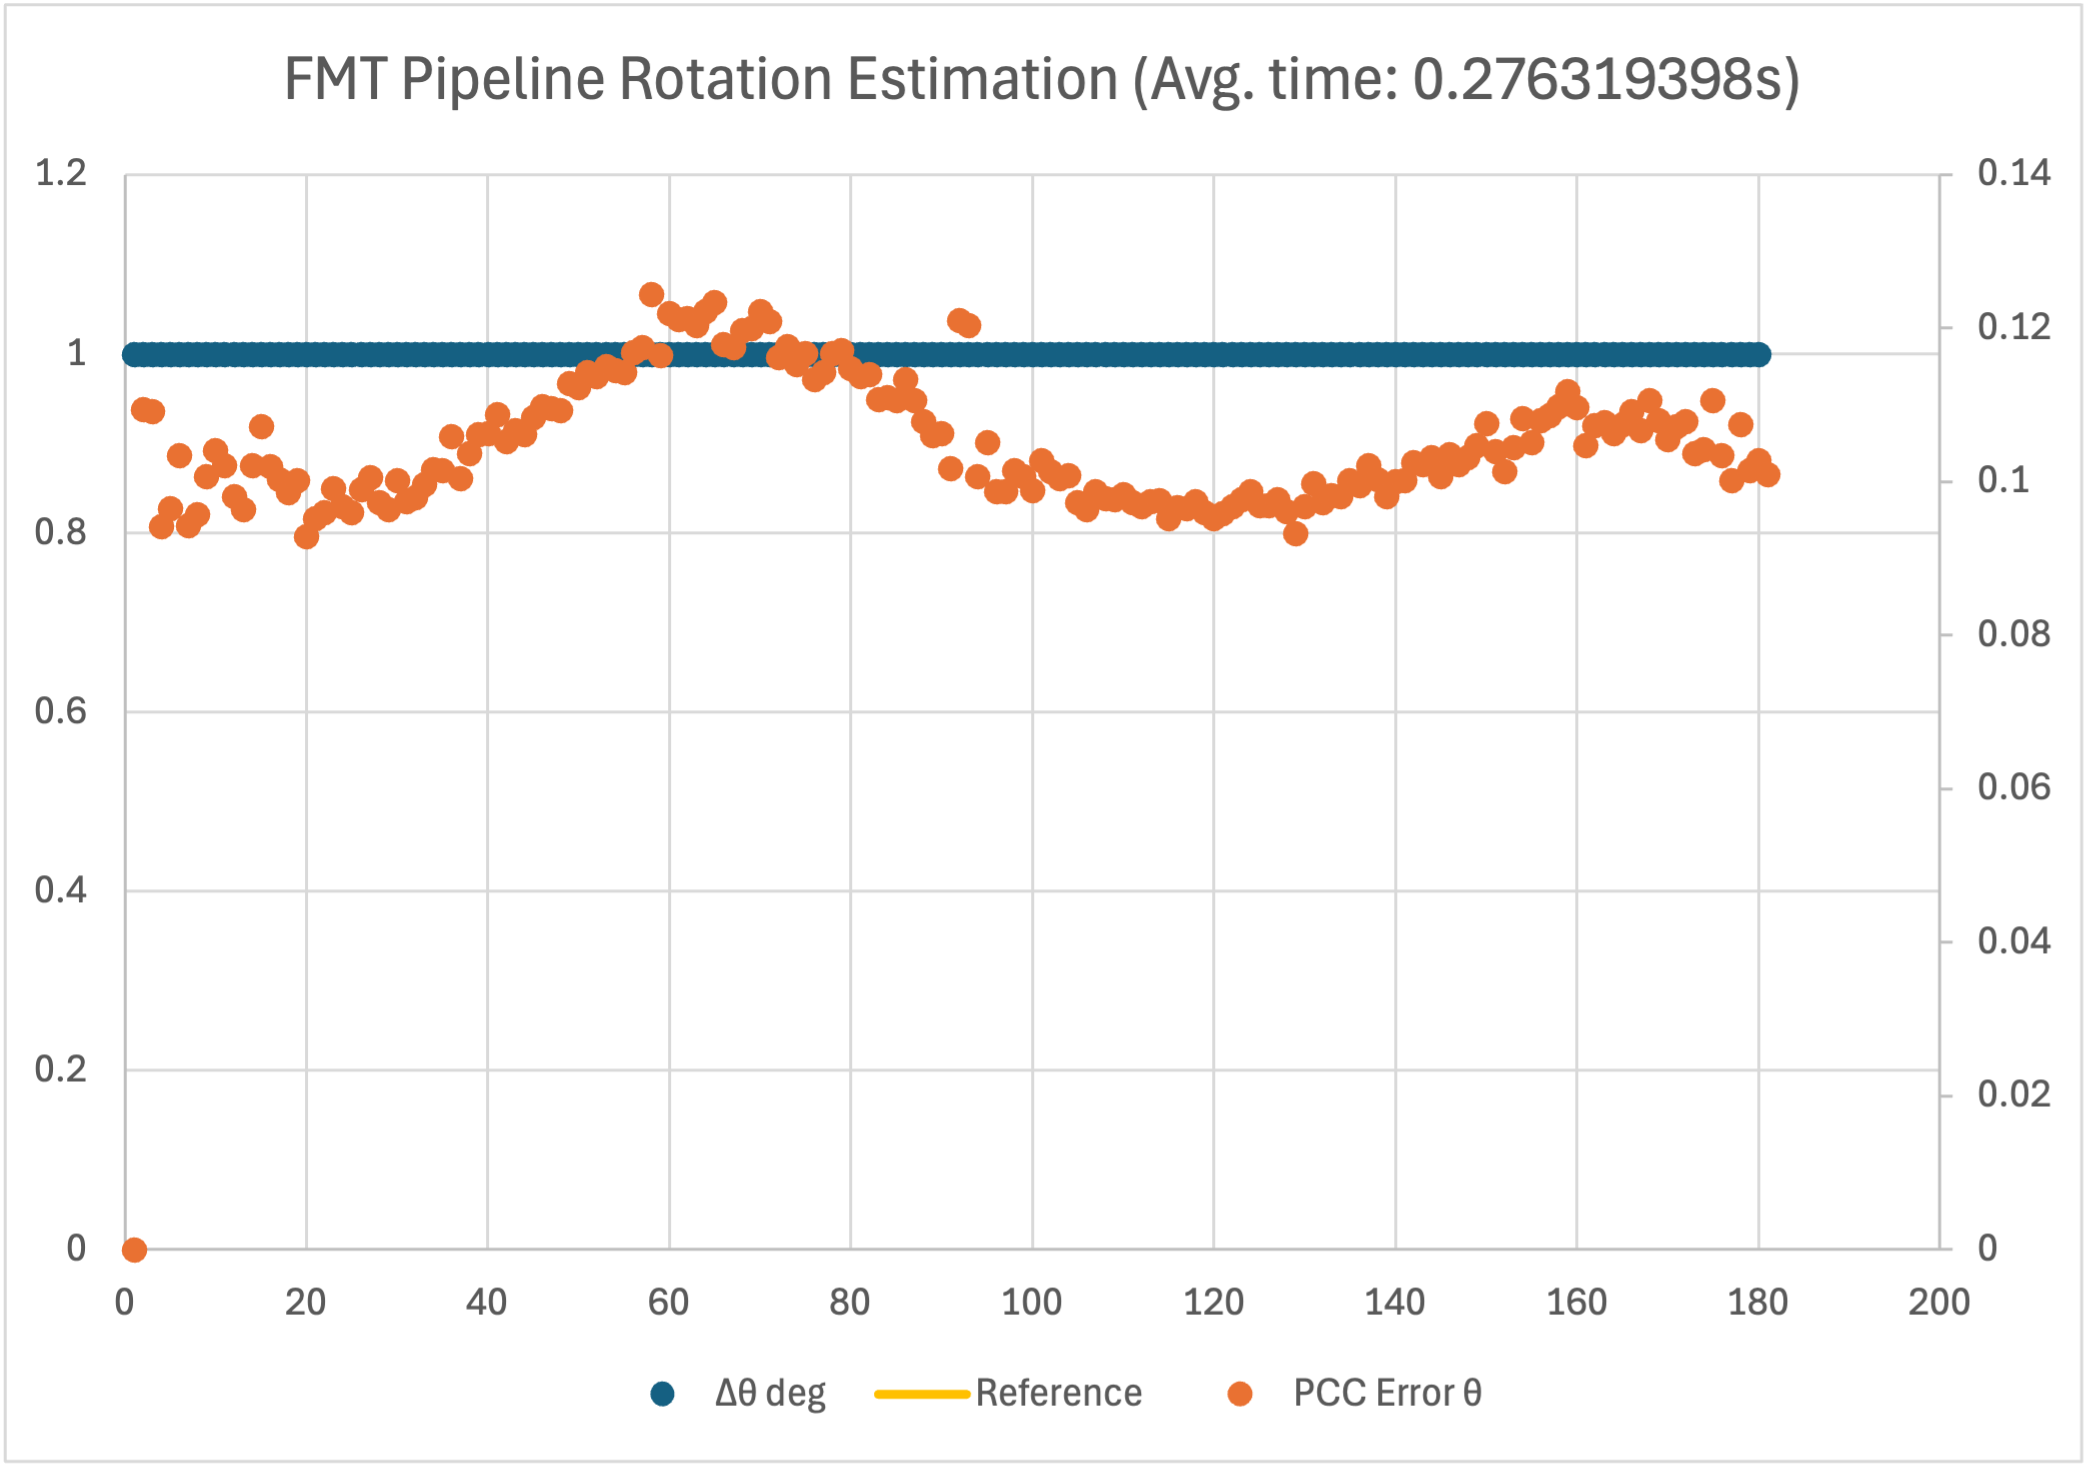
\includegraphics[width=.7\textwidth]{figures/results/rotation-skip-0/PC-Rotation.png}
%   \caption[\citeauthor{Hurtos2015} Pipeline Rotation Estimation]{Rotation estimation using the \citeauthor{Hurtos2015} Phase Correlation Pipeline}
%   \label{fig:pcrotation}
% \end{figure}
\begin{figure}[H]
  \centering
  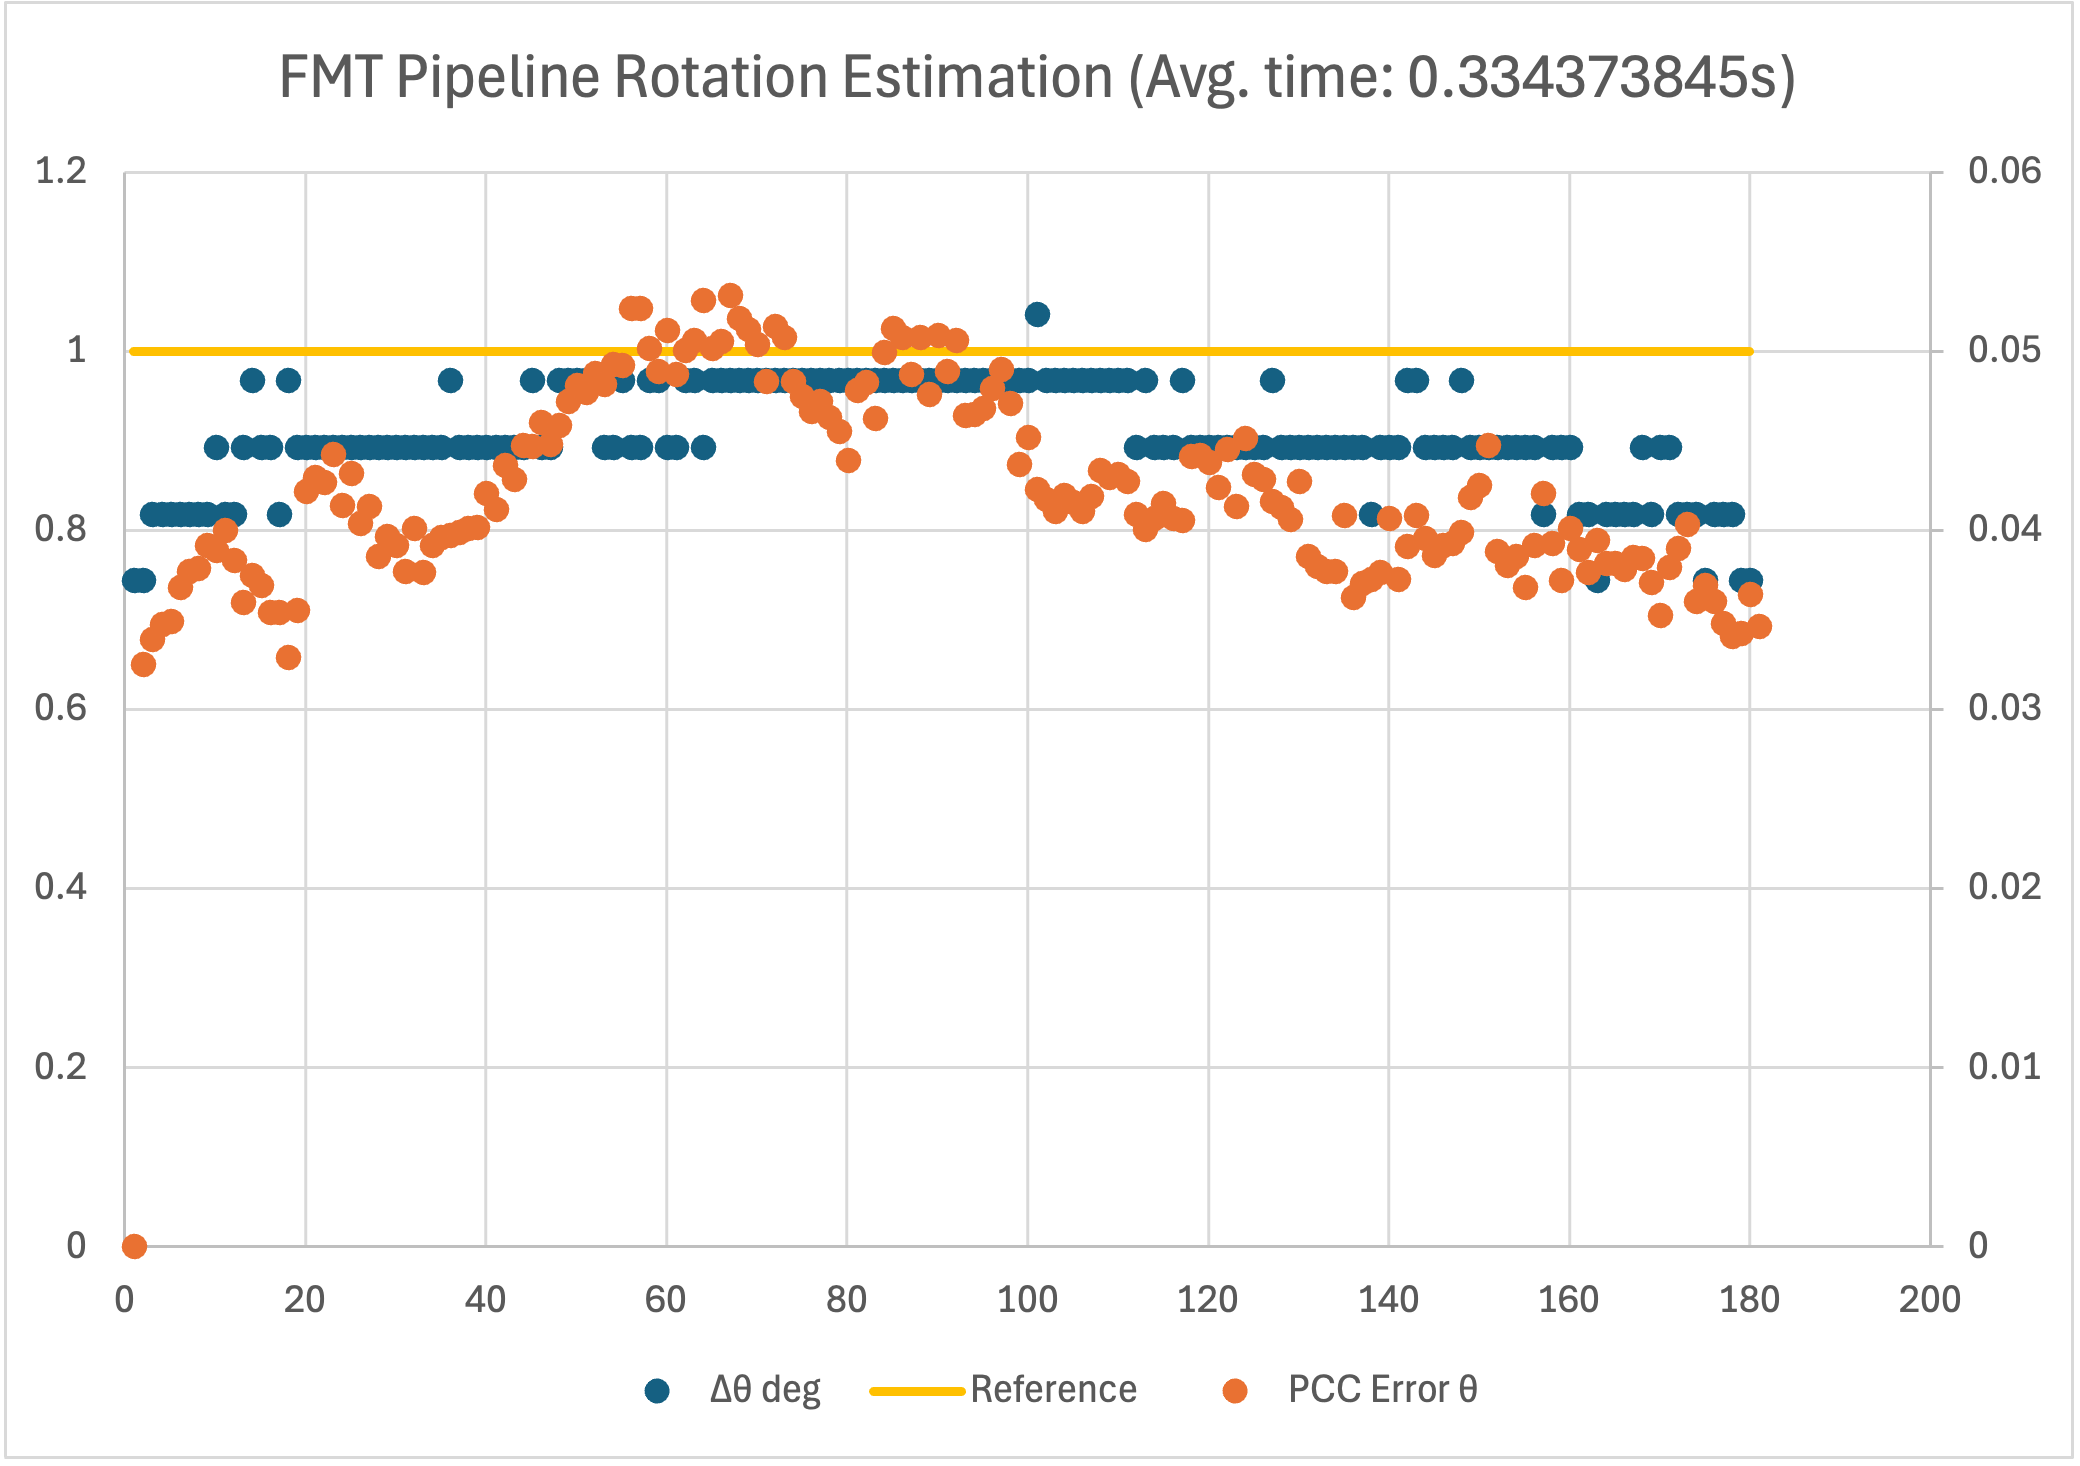
\includegraphics[width=.7\textwidth]{figures/results/rotation-skip-0/FMT-Rotation.png}
  \caption[Fourier-Mellin Pipeline Rotation Estimation Results]{Fourier-Mellin Pipeline Rotation Estimation Results}
  \label{fig:fmresults-skip-0}
\end{figure}


The FMT Pipeline struggled to estimate angles correctly at the beginning and the end of the test set frames. This coincides with frames that extend beyond the edge of the source image and are partially missing information. Counter-intuitively the registration error over these measurements is the lowest, showing a higher degree of confidence when compared to the measurements that were actually closes to the reference value. This is visible in the output \autoref{fig:fmcombined-skip-0}, which is sharpest in the middle where the registrations were closest to the true value, and blurry around the start and end of the semicircle.


\begin{figure}[H]
  \centering
  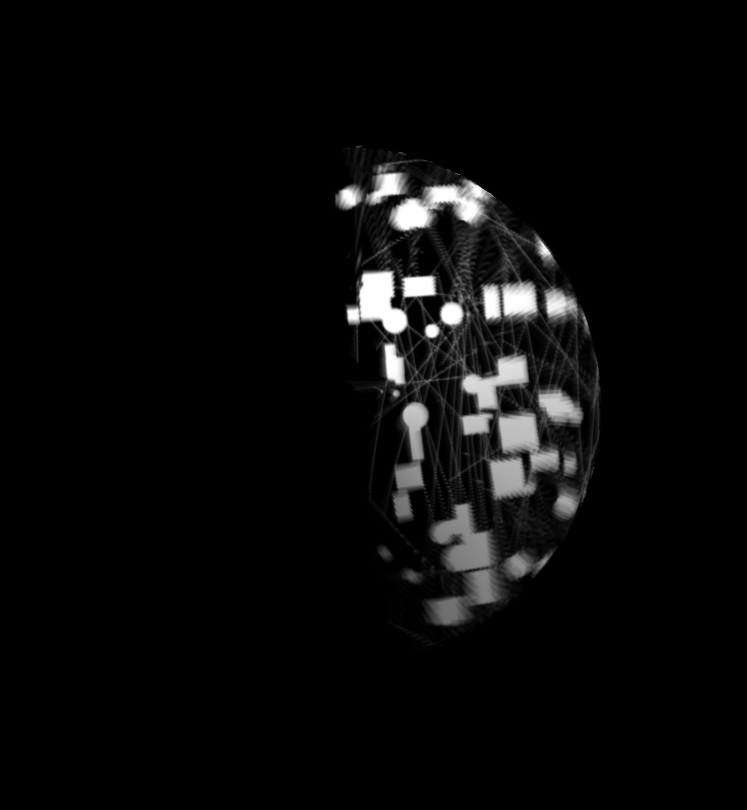
\includegraphics[width=.7\textwidth]{figures/results/rotation-skip-0/FMT.png}
  \caption[Fourier-Mellin Pipeline Rotation Estimation Mosaic]{Fourier-Mellin Pipeline Rotation Estimation Mosaic}
  \label{fig:fmcombined-skip-0}
\end{figure}

\begin{table}[H]
    \centering
    \begin{tabular}{|c|c|}
        \hline
        \textbf{Parameter} & \textbf{Spec} \\ \hline
        Sum of $\Delta\theta$ & 162.9669421º \\ \hline
        Average of $\Delta\theta$ & 0.905371901º \\ \hline
        StdDev of $\Delta\theta$ & 0.059270225º \\ \hline
        Min of $\Delta\theta$ & 0.743801653º \\ \hline
        Max of $\Delta\theta$ & 1.041322314º \\ \hline
        Average Error & 0.094628099º \\ \hline
        Average time & 0.334373845s \\ \hline
    \end{tabular}
    \caption{FMT Pipeline Results}
\end{table}



\begin{figure}[H]
    \centering
    \begin{subfigure}[b]{.45\textwidth}
        \centering
        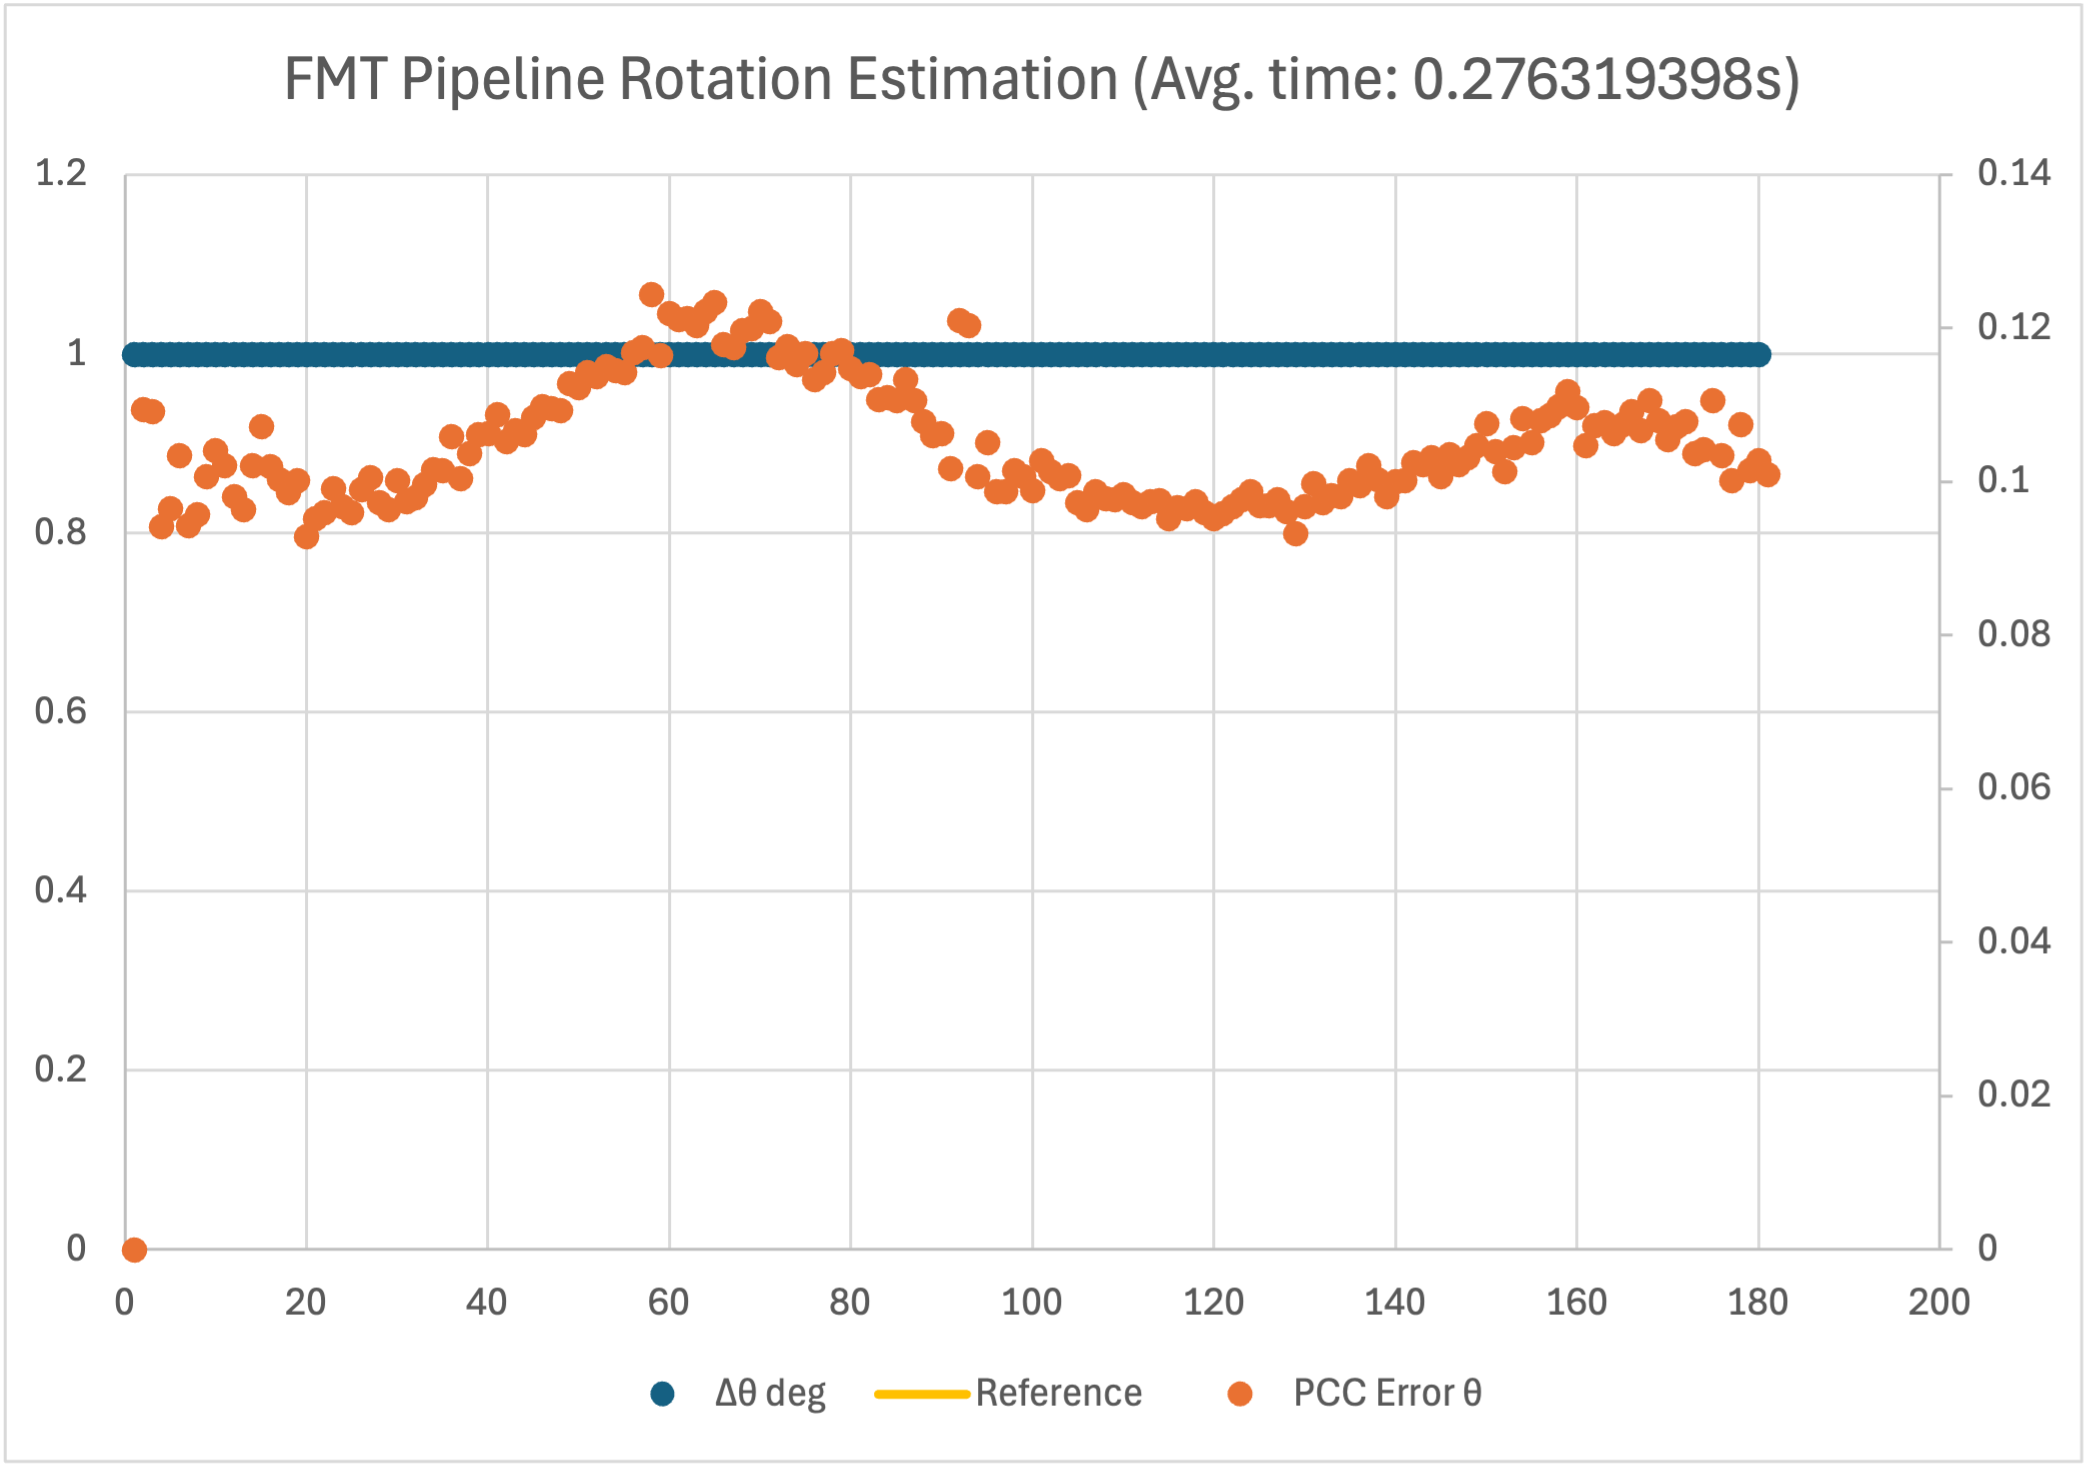
\includegraphics[width=\textwidth]{figures/results/rotation-skip-0/PC-Rotation.png}
        \caption{Rotation estimation}
        \label{sfig:pcrotation}
    \end{subfigure}
    \hfill
    \begin{subfigure}[b]{.45\textwidth}
        \centering
        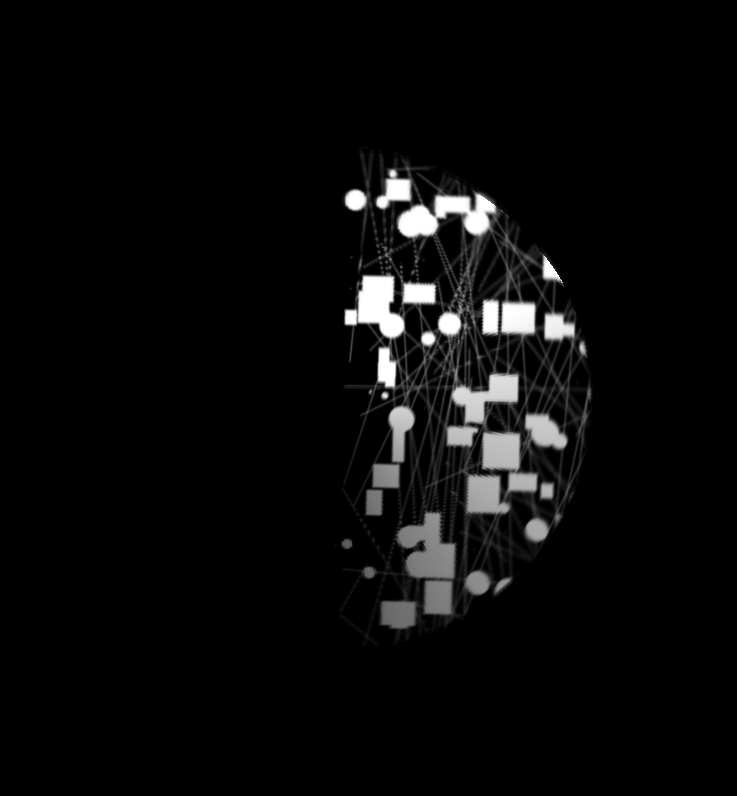
\includegraphics[width=\textwidth]{figures/results/rotation-skip-0/PC.png}
        \caption{Combined image}
        \label{sfig:pccombined-skip-0}
    \end{subfigure}
    \caption[\citeauthor{Hurtos2015} Pipeline Rotation Estimation Results]{Results from running the \citeauthor{Hurtos2015} Pipeline without skipping any frames in between.}
    \label{fig:subfig}
\end{figure}

\begin{table}[H]
    \centering
    \begin{tabular}{|c|c|}
        \hline
        \textbf{Parameter} & \textbf{Spec} \\ \hline
        Sum of $\Delta\theta$ & 180º \\ \hline
        Average of $\Delta\theta$ & 1 \\ \hline
        StdDev of $\Delta\theta$ & 0º \\ \hline
        Min of $\Delta\theta$ & 1º \\ \hline
        Max of $\Delta\theta$ & 1º \\ \hline
        Average Error & 0º \\ \hline
        Average time & 0.334373845s \\ \hline
    \end{tabular}
    \caption{FMT Pipeline Results}
\end{table}

\section{Translation estimation}

\section{Combined estimation}

\section{Effect of downsampling}